\documentclass[12pt]{article}
\usepackage[margin=2.5cm]{geometry}
\usepackage{enumerate}
\usepackage{amsfonts}
\usepackage{amsmath}
\usepackage{fancyhdr}
\usepackage{amsmath}
\usepackage{amssymb}
\usepackage{amsthm}
\usepackage{mdframed}
\usepackage{graphicx}
\usepackage{subcaption}
\usepackage{adjustbox}
\usepackage{listings}
\usepackage{xcolor}
\usepackage{booktabs}
\usepackage[utf]{kotex}
\usepackage{hyperref}

\definecolor{codegreen}{rgb}{0,0.6,0}
\definecolor{codegray}{rgb}{0.5,0.5,0.5}
\definecolor{codepurple}{rgb}{0.58,0,0.82}
\definecolor{backcolour}{rgb}{0.95,0.95,0.92}

\lstdefinestyle{mystyle}{
    backgroundcolor=\color{backcolour},
    commentstyle=\color{codegreen},
    keywordstyle=\color{magenta},
    numberstyle=\tiny\color{codegray},
    stringstyle=\color{codepurple},
    basicstyle=\ttfamily\footnotesize,
    breakatwhitespace=false,
    breaklines=true,
    captionpos=b,
    keepspaces=true,
    numbers=left,
    numbersep=5pt,
    showspaces=false,
    showstringspaces=false,
    showtabs=false,
    tabsize=1
}

\lstset{style=mystyle}

\pagestyle{fancy}
\renewcommand{\headrulewidth}{0.4pt}
\lhead{CSC 369}
\rhead{Worksheet 5 Solution}

\begin{document}
\title{CSC 369 Worksheet 5 Solution}
\maketitle

\bigskip

\begin{enumerate}[1.]
    \item

    \bigskip

    \underline{\textbf{Notes}}

    \begin{itemize}
        \item \textbf{Multi-level Feeback Queue (MLFQ):}

        \begin{itemize}
            \item Is one of the most well-known approaches to scheduling
            \item Does two things:

            \begin{enumerate}[a)]
                \item Optimizes turnaround time
                \item Minimizes response time
            \end{enumerate}

            \item Uses \textbf{priority level} and \textbf{Queues} to achieve it's goal
        \end{itemize}

        \item \textbf{MLFQ Basic Rules:}
        \begin{itemize}
            \item Jobs on same queue $\to$ Same priority
            \item \textbf{Rule 1:} If $\text{Priority(A)} > \text{Priority(B)}$, A runs (B doesn't)
            \item \textbf{Rule 2:} If $\text{Priority(A)} = \text{Priority(B)}$, A \& B run in RR
        \end{itemize}

        \bigskip

        \begin{center}
        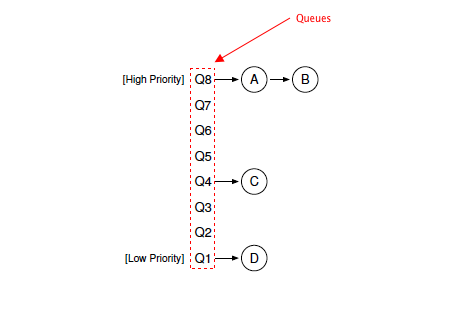
\includegraphics[width=0.8\linewidth]{images/worksheet_5_solution_1.png}
        \end{center}

        \item \textbf{Attemp \#1: How to Change Priority}

        \begin{itemize}
            \item \textbf{Rule 3:} When a job enters the system, it is placed at the \underline{highest}
            priority (the topmost queue)
            \item \textbf{Rule 4a:} If a job uses up an entire time slice while running , its' priority is
            \underline{reduced} (i.e. it moves down on queue).
            \item \textbf{Rule 4b:} If a job gives up the CPU before the time slice is up, it stays
            at the \underline{same} priority level (e.g I/O Operation)

            \bigskip

            \underline{\textbf{Example (Shortest Running Job):}}

            \bigskip

            \begin{enumerate}[1)]
                \item A job $A$ enters system
                \item Job is placed on highest Queue $Q_2$
                \item After time-slice (e.g. 10 ms) in $Q_2$, $A$ is placed on lower queue $Q_1$
                \item After time-slice in $Q_1$, $A$ is placed in lowest priority queue $Q_0$
            \end{enumerate}
        \end{itemize}


    \end{itemize}
\end{enumerate}

\end{document}